\documentclass[UTF8,11pt]{ctexart}
\usepackage[a4paper,margin=2.35cm]{geometry}
\usepackage{amsmath,amssymb,amsthm,booktabs,graphicx,float,array}
\usepackage[colorlinks=true,allcolors=blue]{hyperref}
\usepackage[font=small,labelfont=bf]{caption}
\graphicspath{{../figures/}}
\newtheorem{proposition}{命题}
\newtheorem{theorem}{定理}
\newtheorem{corollary}{推论}
\newcommand{\nrmse}{\operatorname{NRMSE}}
\newcommand{\indet}{\textsc{Indeterminate}}
\title{稀疏多通道数据中共享有限记忆实现的证据门控识别与主动拒绝}
\author{段海涛$^{1,*}$，胡宁$^{2}$，李书群$^{3}$，胡初扬$^{4}$\\[2mm]
\small $^1$杭州电子科技大学计算机学院，中国杭州\\
\small $^2$杭州电子科技大学机械工程学院，中国杭州\\
\small $^3$西交利物浦大学数学物理学院，中国苏州\\
\small $^4$加州大学圣克鲁兹分校计算机科学与工程系，美国加利福尼亚州圣克鲁兹 95064\\[1mm]
\small $^*$通讯作者：\href{mailto:duanhaitao@hdu.edu.cn}{duanhaitao@hdu.edu.cn}}
\date{}

\begin{document}
\maketitle

\begin{abstract}
有限衰减模态之和广泛用于表征遗传动力学，但良好拟合并不能证明所识别模态具有可辨识性和跨样本可迁移性。本文提出一种证据门控协议，用于从稀疏多通道观测中选择数据所支持的最小共享有限记忆实现；当预测充分性与可辨识性不一致时，协议主动拒绝机制阶数结论。正衰减率由独立实验单元共享，幅值与偏置保持单元特定。候选阶数由信息改善、留出单元的前段到后段预测、跨折衰减率稳定性和相邻衰减率分离共同判定。高斯两点定理给出相邻衰减率不可区分边界，独立推论则说明校准拒绝门获得条件一致性所需的假设。由不相交半合成数据校准的阈值，在四类噪声生成器下均接受 40/40 个分离试验并拒绝 40/40 个合并试验；每类生成器的 Wilson 95\% 下界为 0.9124，因此该结果仍是设计条件下的证据，而不是普适保证。在四个冻结压力记录中，移除唯一失败门均会改变判决，说明这些门在所选记录上并非冗余。四个相互独立的公开应用域提供互补检验：完整观测窗的 PVA 应力松弛支持三阶有限经验实现；覆盖 9 个材料组的 17 次铜合金应力松弛试验在 AR(1) 剖面 BIC 下支持共享一阶经验实现；气敏恢复的三阶模型预测较好但衰减率合并，因此结论为 \indet{}；在覆盖三种冷却器状态的 30 个液压负载循环上，BIC 偏好二阶，但留出状态 NRMSE 从 0.23780 恶化至 0.51128，局部边界指数降至 0.057，协议再次拒绝。两个拒绝任务在全部 27 组阈值设置下均保持无法判定。研究由此区分预测改善、有限表示与机制识别，并提供版本化 Python 接口和机器可读决策记录。
\end{abstract}

\noindent\textbf{关键词：}记忆实现；松弛谱；可辨识性；模型阶数选择；不确定性感知拒绝；科学机器学习

\section{引言}
具有遗传效应的系统常被压缩表示为有限指数项之和。该表示连接了松弛谱、有理逼近、辅助状态模型和非马尔可夫降阶动力学。经典 Prony 恢复和向量拟合提供了有效的重构方法 \cite{stampfer2020gop,gustavsen1999vector,bosner2021parallel}，近年的广义朗之万模型则从轨迹中学习更具表达力的记忆核 \cite{lei2016parameterization,ge2024state,lang2026learning}。本文关注的问题不同：有限、含噪且具有分组结构的观测何时足以支持某个最小共享实现，何时应当拒绝指定机制阶数？

仅选择残差最小的曲线并不足够。额外模态可能吸收噪声，彼此接近的衰减率可能在局部不可区分，而能够预测留出观测的模型仍可能具有无法解析的内部谱。当同一实验中的多个通道被错误当作独立重复，或者观测窗未覆盖渐近尾部时，这些问题会进一步加剧。因此，模型支持需要同时考虑拟合、迁移、稳定性和可分离性，而不能依赖单一评分。

本文构建联合识别--拒绝协议，并作出四项贡献。第一，定义共享衰减率、单元特定幅值的有限实现模型，以四个预先声明的证据门选出最小受支持阶数。第二，引入显式 \indet{} 输出，防止将预测增益自动提升为机制结论。第三，绘制观测设计边界，并将其与残差相关性及衰减率灵敏度条件数联系起来。第四，将协议实现为具有稳定 \texttt{fit}、\texttt{evaluate}、\texttt{decide} 和 \texttt{report} 操作的软件契约。

四个公开任务分别检验不同层面的主张。PVA 与铜合金应力松弛数据用于检验跨物理试件或材料组迁移 \cite{schelkow2026pva,kupferdigital2024relaxation}；气敏数据用于检验跨采集批次迁移，并将同次暴露内的传感器通道保留为聚类观测 \cite{ziyatdinov2015dataset,ziyatdinov2015bioinspired}；液压系统数据用于检验受控部件状态间的多通道冷却瞬态迁移 \cite{helwig2018hydraulic}。两个受支持的经验实现与两类拒绝结果共同构成主要证据，使协议能够区分观测实际识别的结构与仅由样本内评分偏好的近似。

\section{相关工作与贡献边界}
有限指数和有理表示具有长期的数值研究基础。广义 Prony 方法可恢复稀疏特征函数展开并分析重构敏感性 \cite{stampfer2020gop}；矩阵铅笔变体将恢复扩展到多变量观测 \cite{bosner2021parallel}；向量拟合则从频域响应估计共享极点 \cite{gustavsen1999vector}。本文将这些方法作为表示基础和对照方法，不提出新的 Prony 求解器，也不声称可从含噪数据中实现精确恢复。

在数据驱动非马尔可夫建模中，有理辅助状态参数化和学习型记忆核已经能够支撑准确的降阶动力学 \cite{lei2016parameterization,ge2024state,lang2026learning}。这些工作的主要目标是记忆核估计或动力学预测。本文的目标是判断独立实验单元共同支持的最小有限实现，并在数据无法区分候选机制时输出拒绝结论。

作者此前的 DFSC 工作将可微 Mittag--Leffler 传播子实现为科学机器学习基元 \cite{hu2026dfsc}，其贡献集中于可微传播、数值控制和软件组合。本文既不扩展该求值器，也不把其软件实现作为统计结论的来源，而是处理一个不同的推断问题：分组观测是否足以识别共享有限记忆实现。该边界避免把“已有可用软件”误解为“机制已经可辨识”。

松弛谱识别同样是黏弹性中的经典逆问题，正则化与时间尺度选择可提高谱恢复的稳定性 \cite{stankiewicz2023relaxation}。本文协议对这些估计器形成补充：它要求留出单元预测、跨折衰减率稳定性以及衰减率分离。因此，创新点在联合判定契约，而不在任一单独判据。

相邻指数模态的分辨率还受到 Vandermonde 型系统条件数和超分辨率极限的约束 \cite{moitra2015superresolution}。模型阶数惩罚通常采用 BIC \cite{schwarz1978bic}，而含相关残差的小样本时间序列需要额外敏感性分析 \cite{hurvich1989timeseries}。本文不把任一准则视为机制证明，而是把信息准则、迁移、稳定性和局部分离组织为可审计的联合证据。
经典模型阶数研究明确区分信息准则、预测选择与贝叶斯证据，而不把它们视为等价判据 \cite{stoica2004modelorder,shao1993crossvalidation,kass1995bayes}。选择性预测研究也把“证据不足时拒绝输出”形式化为明确决策 \cite{geifman2017selective}。本文拒绝的是共享动力学阶数解释，而不是单个样本的类别预测；这些工作为显式拒绝状态提供方法学背景，四门控的分组动力学审计则是本文针对当前问题的设计。

\section{模型与证据契约}
\subsection{共享有限实现}
对实验单元 $i$ 在时刻 $t_{ij}$ 的观测，候选 $r$ 阶模型写为
\begin{equation}
y_i(t)=c_i+\sum_{k=1}^{r}a_{ik}\exp(-\lambda_k t)+\varepsilon_i(t),
\qquad a_{ik}\in\mathbb R,\quad 0<\lambda_1<\cdots<\lambda_r.
\label{eq:model-zh}
\end{equation}
衰减率 $\lambda_k$ 在实验单元之间共享，幅值 $a_{ik}$ 和偏置 $c_i$ 则由单元决定。该分解将候选公共谱与实验尺度和基线差异分开。其适用范围限于已声明的、正有限指数松弛具有合理解释的时间区间。

\subsection{四个证据门}
候选阶数 $r=1,\ldots,r_{\max}$ 使用训练单元拟合。只有同时通过以下四个证据门的最小阶数才被支持。

\paragraph{信息门。} 设拟合观测数为 $n$，自由参数数为 $q_r$，定义
\begin{equation}
\mathrm{BIC}_r=n\log(\mathrm{SSE}_r/n)+q_r\log n,
\end{equation}
并要求相对低阶模型达到预先声明的信息改善幅度 \cite{schwarz1978bic}。由于松弛曲线残差通常具有序列相关性，最终审计同时报告高斯 AR(1) 剖面 BIC 与有效样本量诊断。两种准则一致时可作为支持证据；若其阶数排序不一致，则报告敏感性，而不在观察结果后重新选择阈值 \cite{hurvich1989timeseries}。

\paragraph{迁移门。} 完整实验单元被留出。先用其余单元学习衰减率，再用留出曲线前 60\% 标定幅值，并预测后 40\%。误差定义为
\begin{equation}
\nrmse_i=\frac{\|\hat{\mathbf y}_{i,\mathrm{late}}-\mathbf y_{i,\mathrm{late}}\|_2}
{\|\mathbf y_{i,\mathrm{late}}-\bar y_{i,\mathrm{late}}\mathbf 1\|_2+\epsilon}.
\end{equation}

\paragraph{稳定性门。} 各折的对数衰减率必须保持稳定，每个模态的 $\log\lambda_k$ 跨折标准差不得超过冻结阈值。

\paragraph{分离门。} 相邻衰减率必须满足
\begin{equation}
\min_k\frac{\lambda_{k+1}}{\lambda_k}\ge \rho_{\min}>1.
\label{eq:separation-zh}
\end{equation}
该门避免把残差有所降低、但谱线已经合并的拟合解释为不同时间尺度。

若没有阶数通过全部证据门，则输出 \indet{}。这不表示优化失败，而是记录当前声明域中的观测不足以支持所要求的机制分辨率。

\begin{figure}[H]
\centering
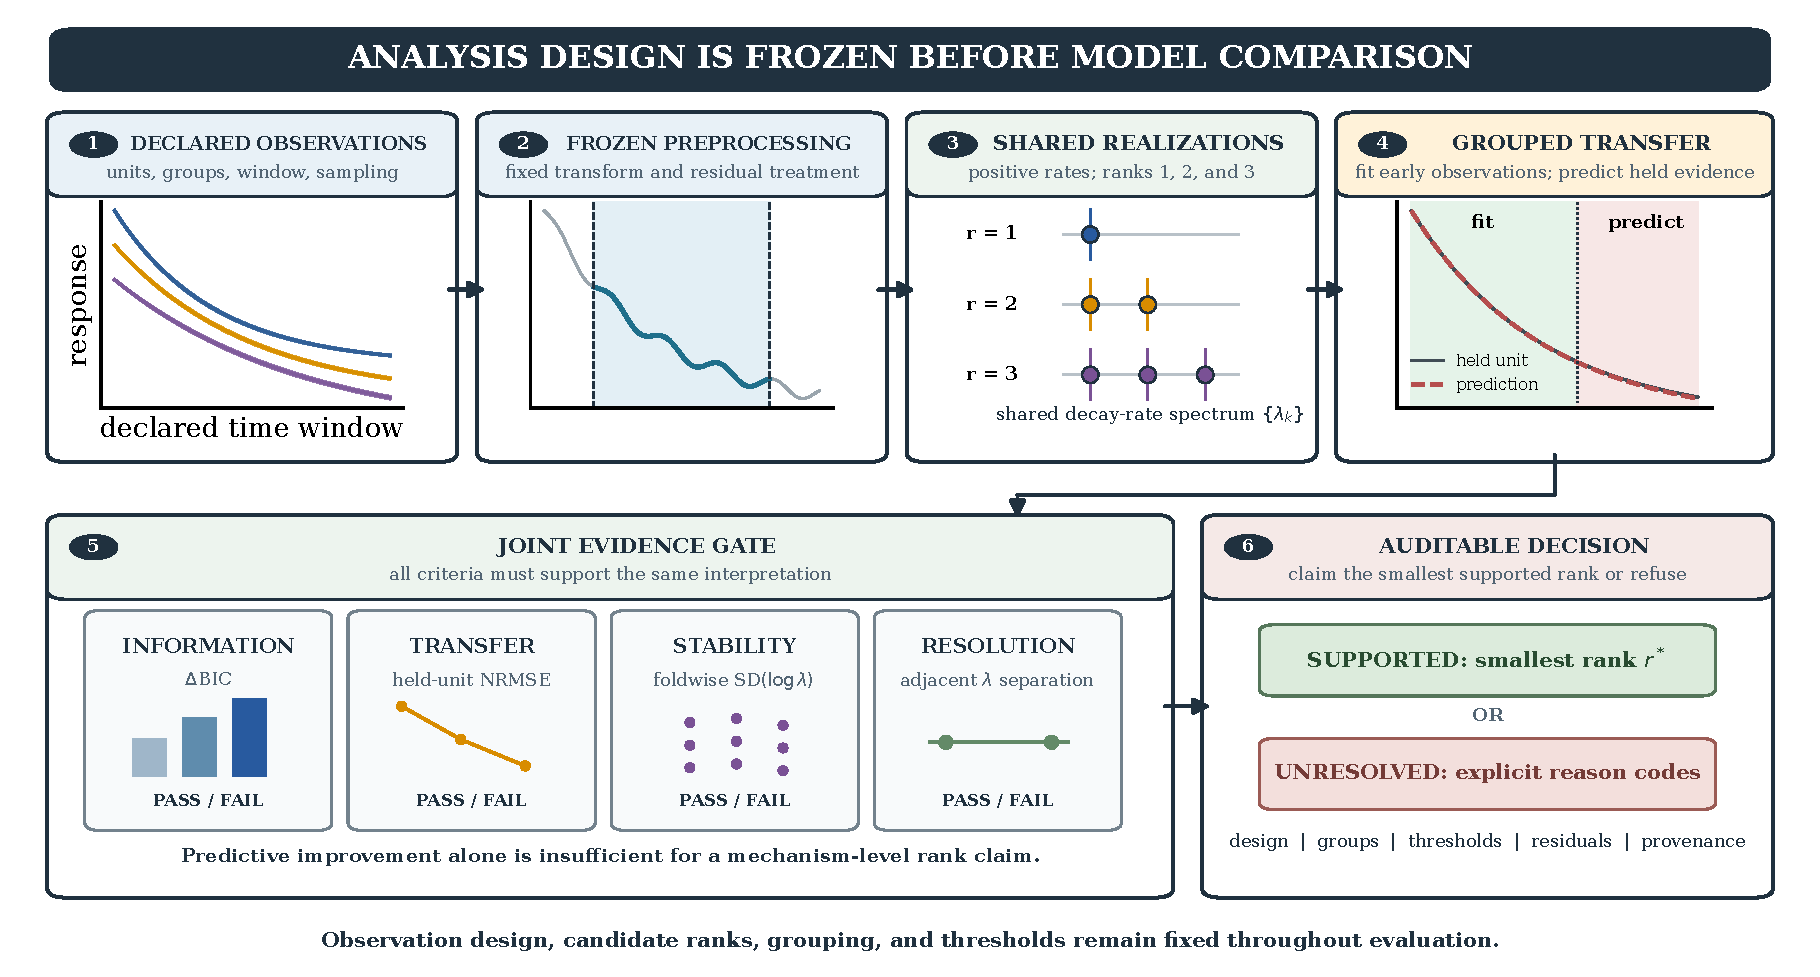
\includegraphics[width=0.96\textwidth]{fig_stage62_method_workflow.pdf}
\caption{冻结分析流程。判定以独立实验单元为层级，而不是以单个通道或重复采样点为层级。}
\label{fig:workflow-zh}
\end{figure}

\subsection{最小可辨识性分析}
令 $\boldsymbol\mu(\theta)$ 为堆叠均值响应，$J=\partial\boldsymbol\mu/\partial\theta$。在投影消除幅值和偏置等干扰参数后，衰减率对应的 $J$ 列向量必须保持线性无关，才能获得局部识别。

\begin{proposition}[局部衰减率识别]
若投影后的衰减率灵敏度矩阵 $J_\lambda$ 在 $\theta^\star$ 处满列秩，则共享衰减率在 $\theta^\star$ 的邻域内局部可辨识。当其最小奇异值趋近于零时，局部不确定性发散，彼此接近的衰减率无法稳定解析。
\end{proposition}
\begin{proof}
满列秩使局部 Fisher/Gauss--Newton 矩阵 $J_\lambda^\top WJ_\lambda$ 对任意正定 $W$ 均为正定。逆函数论证给出局部单射性；最小奇异值消失时，逆灵敏度无界。
\end{proof}

对于两个接近的衰减率 $\lambda$ 与 $\lambda+\delta$，均值定理给出
\begin{equation}
|e^{-\lambda t}-e^{-(\lambda+\delta)t}|
\le |\delta|t e^{-\min(\lambda,\lambda+\delta)t}.
\label{eq:coalescence-zh}
\end{equation}
因此，在有限含噪观测窗中，即使双模态模型降低了残差，也可能无法区分两个模态。式~\eqref{eq:coalescence-zh} 支撑分离门，$J_\lambda$ 的奇异谱则提供连续诊断。

原始采样数本身不是信息量。在残差协方差为 $\Sigma$ 时，局部信息为 $J^\top\Sigma^{-1}J$。延长观测窗会同时改变灵敏度几何和残差相关性；增加采样密度也可能只增加近似重复的矩阵行。因此，支持边界不必随采样点数单调变化。

相邻衰减率的极限可以进一步形式化。考虑方差为 $\sigma^2$ 的独立高斯观测，备择模型包含 $a_i e^{-\lambda t}+b_i e^{-(\lambda+\delta_n)t}$，相应低一阶合并模型采用 $(a_i+b_i)e^{-\lambda t}$。定义
\begin{equation}
R_n^2=\frac{\delta_n^2}{\sigma^2}\sum_{i,\ell}b_i^2t_{i\ell}^2
e^{-2\min(\lambda,\lambda+\delta_n)t_{i\ell}}.
\label{eq:boundary-index-zh}
\end{equation}

\begin{theorem}[高斯相邻衰减率不可区分性]
在上述高斯模型下，$\mathrm{KL}(P_{r,n}\|P_{r-1,n})\le R_n^2/2$。若 $R_n\to0$，任意可测阶数检验均满足 $\alpha_n+\beta_n\to1$，因而不存在沿该设计序列一致区分相邻模态的阶数判定。
\end{theorem}
\begin{proof}
两模型在观测 $(i,\ell)$ 处的均值差为 $d_{i\ell}=b_i[e^{-(\lambda+\delta_n)t_{i\ell}}-e^{-\lambda t_{i\ell}}]$。由式~\eqref{eq:coalescence-zh} 可将 $\|d\|_2^2/\sigma^2$ 上界为 $R_n^2$，共同协方差高斯分布的公式随即给出 KL 上界。Pinsker 不等式与两点检验下界给出 $\alpha_n+\beta_n\ge1-\operatorname{TV}(P_{r,n},P_{r-1,n})\ge1-R_n/2$ \cite{tsybakov2009nonparametric}。
\end{proof}

\begin{corollary}[多衰减率模型中的嵌入式障碍]
若除一对相邻衰减率外的其他衰减率与干扰参数均固定，或其估计误差为 $o(R_n)$，则 $r$ 阶模型与合并后的 $(r-1)$ 阶模型包含上述定理的两点子试验。因此当 $R_n\to0$ 时，在更大的参数类上也不存在一致阶数检验。
\end{corollary}
\begin{proof}
将较大参数空间限制到定理使用的两个分布。若较大空间上存在一致检验，则其在该两点限制上也一致，与定理矛盾。
\end{proof}
\begin{corollary}[校准诊断量的条件性拒绝]
设某一固定观测设计上的诊断量 $\widehat R_n$ 满足 $|\widehat R_n-R_n|=o_p(c_n)$，其中 $c_n\downarrow0$，且阈值仅由与评估样本独立的校准数据确定。若 $R_n=o(c_n)$，则规则 $\widehat R_n\le c_n$ 以概率趋于一输出 \indet{}。若相邻衰减率保持固定分离、投影信息最小特征值发散、参数估计一致且其余证据门一致，则该规则以概率趋于一接受真实阶数。
\end{corollary}

这些结果只属于局部或嵌入式结论，不证明非线性核、不规则观测、非高斯噪声或联合漂移干扰参数下的全局可辨识性。软件实现报告局部代理量 $\widehat D$：先将对数衰减率灵敏度投影到单曲线偏置和幅值列的正交补，再以最小投影奇异值乘最小相邻对数间隔并除以残差噪声；进一步除以观测数平方根以移除其主导样本量缩放。除非另加假设，这两个版本都不是 $R_n$ 的估计量。因此，本文只在预先声明的半合成设计上校准归一化代理量，并在不相交的种子上评估；它是任务内部诊断量，而不是通用阈值。

\subsection{超出正实完全共享衰减率的声明扩展}
在不改变四个公开数据集冻结判决的前提下，本文额外检验四项有明确范围的扩展。稳定振荡记忆采用实数共轭极点块表示：
\begin{equation}
y_i(t)=c_i+\sum_k a_{ik}e^{-\lambda_k t}+\sum_j e^{-\gamma_j t}\{u_{ij}\cos(\omega_jt)+v_{ij}\sin(\omega_jt)\}+\epsilon_i(t),
\label{eq:oscillatory-extension-zh}
\end{equation}
其中 $\gamma_j,\omega_j>0$。部分共享模型设 $\log\lambda_{gk}=\mu_k+\delta_{gk}$、$\sum_g\delta_{gk}=0$，并加入声明的二次惩罚 $\eta\sum_{g,k}\delta_{gk}^2$；$\eta$ 不得利用最终证据组选择。稠密对数正态松弛测度用于检验有限衰减和假设的类外失配。组级 conformal 审计则对每个独立校准组只计算一个非一致性分数。对 $m$ 个可交换校准组，其上侧阈值取第 $\lceil(m+1)(1-\alpha)\rceil$ 个次序统计量（最高截为 $m$），上尾检验值为 $(1+\#\{S_j\ge S_{\rm test}\})/(m+1)$ \cite{shafer2008conformal}。该结论只是在组可交换条件下的有限样本边际保证，不是组分布偏移后的分布无关保证。
\section{公开数据集与冻结协议}
\subsection{PVA 应力松弛}
第一项任务使用圆柱形 PVA 凝胶聚合物电解质样品的公开应力松弛数据 \cite{schelkow2026pva}。数据包含三个试件，每个试件有三个循环。分析不使用平滑处理，采用留一试件折学习共享衰减率。完整任务的观测窗为 28 秒，每条曲线保留 96 个点。由于独立试件仅有三个，曲线层级的不确定性汇总只作描述性证据，不被解释为总体推断。

\subsection{铜合金应力松弛}
第二项任务采用公开的 KupferDigital 力学试验档案 \cite{kupferdigital2024relaxation}。17 个物理应力松弛试验文件来自 9 个材料代码组，每个文件视为一个独立实验单元。工程应力除以首个登记应力，随后在声明的 24 小时试验范围内，从零到所有完整曲线最短终点登记到共同的 96 点网格，不作平滑。验证时留出完整材料代码组，因此同一材料组的重复试件不会跨折。该判定只涉及声明曲线上的共享经验松弛实现，不被解释为唯一微观机制的证据。

\subsection{气敏恢复过程}
第三项任务采用 UCI 数据集 308 \cite{ziyatdinov2015dataset}。从五个采集批次中保留 50 次非空气暴露实验，每次实验包含 16 个金属氧化物传感器通道。分析限制在预先登记的 180--300 秒恢复区间，并按 12 秒物理调制周期计算中位数。通道始终聚类在对应暴露实验内，验证时留出完整采集批次。全部阈值及 60/40 标定--预测切分均在拟合前冻结。

\subsection{液压冷却瞬态}
第四项任务采用 UCI 数据集 447，该数据来自液压试验台重复执行的 60 秒负载循环 \cite{helwig2018hydraulic}。选择该数据是为了利用其受控状态、重复循环和聚类传感器进行外部多通道动态压力测试，并不把它作为部件级松弛机制的物理验证。实验固定阀门状态、泵泄漏、蓄能器压力和稳定标志，仅改变冷却器效率（3\%、20\% 和 100\%），每种状态保留 10 个独立循环。分析冷却效率、冷却功率和两个温度通道在第 20--55 秒的响应，不作平滑。归一化只使用声明观测窗的前 22 个样本。验证时留出完整冷却器状态，四个通道始终聚类在所属循环内。

\subsection{基线与统计审计}
气敏任务将共享衰减率模型与独立非线性三阶拟合、固定网格非负最小二乘（NNLS）及 Prony 递推基线比较；液压任务另加入拉伸指数、AR(2)、Prony 与固定网格 NNLS 的前段标定--后段预测对照。铜合金任务采用留一材料组预测、普通 BIC 与 AR(1) 剖面 BIC 敏感性分析比较候选阶数。所有方法采用相同的任务内切分。配对或分组比较以独立暴露实验、负载循环、试件或试验文件为单元，不把单元内通道与重复采样计作独立样本。稳健性检查包括聚类 Bootstrap 区间、单侧配对 Wilcoxon 检验、1/2/4/8 多起点、留一组迁移和 $3\times3\times3$ 阈值网格。基线 $p$ 值在每个公开任务的比较族内分别采用 Holm 逐步法校正，以控制族错误率。阈值扫描只用于敏感性审计，不用于观察结果后的阈值选择。

\section{结果}
\subsection{证据层级}
本文按三层解释证据。第一层为生成阶数已知的半合成对照，用于检验声明噪声过程下的决策行为；第二层为公开分组数据，用于检验有限经验实现、迁移、稳定性与拒绝，但并不提供微观阶数真值；第三层的机制真值需要独立物理标签或干预，本文不作此类主张。因此，公开数据上的受支持阶数表示通过冻结契约的最小有限实现，\indet{} 则表示该契约下证据不足。

\subsection{校准正例与拒绝对照}
分组半合成实验提供已知阶数对照。归一化局部边界阈值采用与评估数据不相交的校准切分，并以几何中点固定为 0.49085。该阈值不再调节，直接在独立同分布高斯、AR(1)、AR(2) 和异方差四类噪声下评估。对真实衰减率 $(0.12,0.72)$ 明确分离的二阶系统，每类噪声均接受 40/40 次；对真实衰减率 $(0.34,0.37)$ 合并的二阶系统，每类噪声均拒绝 40/40 次。每个观察比例均为 1.00，其双侧 Wilson 95\% 区间为 $[0.9124,1]$。这些试验只量化对四类声明噪声生成器的迁移，不是任意残差过程上的普适错误率或覆盖率保证。

\begin{figure}[H]
\centering
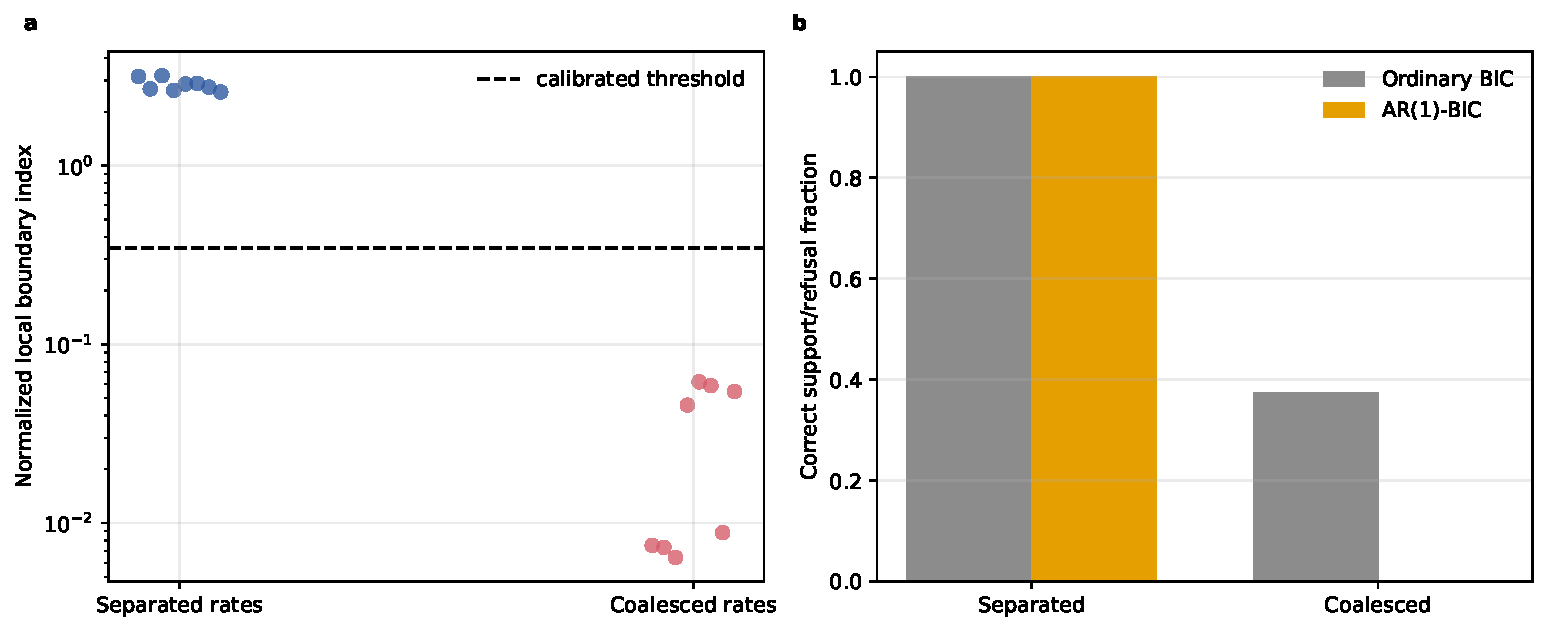
\includegraphics[width=0.90\textwidth]{fig_stage65_acceptance_calibration.pdf}
\caption{使用不相交校准种子和评估种子的半合成校准。（a）归一化局部边界代理量分离了预先声明的“明确分离”与“合并”设计。（b）普通 BIC 与 AR(1) 剖面 BIC 的正确支持或拒绝情况；由于信息准则本身常把未解析的相邻衰减率合并为低阶表示，因此仍需显式边界门。}
\label{fig:semisynthetic-zh}
\end{figure}
\subsection{逐门移除的决策审计}
我们在不重新拟合的前提下，对冻结压力记录重新应用判决规则。PVA 边界记录分别提供“仅迁移门失败”和“仅稳定门失败”的过渡；UCI 气敏记录提供“仅分离门失败”的过渡；另以信息增益为负、其他检查均通过的受控过渡审计信息门逻辑。完整契约在四种情形下均拒绝或保留低阶；移除唯一失败门后，四种情形均提升到更高阶。这说明四个门并非冗余的布尔拼接。该结果只证明所选冻结压力记录上的逻辑相关性，不估计总体层面的变量重要性。
\subsection{PVA 独立支持及其边界}
在完整 28 秒任务上，协议返回 \texttt{SUPPORTED\_RANK\_3}。表~\ref{tab:pva-zh} 显示三阶模型具有最低 BIC 和留出曲线 NRMSE，同时满足衰减率稳定性和分离门。

\begin{table}[H]
\centering
\caption{冻结协议下的 PVA 公开数据结果。}
\label{tab:pva-zh}
\begin{tabular}{rrrr}
\toprule
阶数 & 平均 BIC & 留出 NRMSE 中位数 & 最大跨折对数衰减率标准差\\
\midrule
1 & $-6944.806$ & 0.01757 & 0.0284\\
2 & $-8350.562$ & 0.01121 & 0.1540\\
3 & $-8670.737$ & 0.00932 & 0.3685\\
\bottomrule
\end{tabular}
\end{table}

三阶相对一阶的曲线误差中位改善为 48.4\%，描述性 Bootstrap 区间为 [39.5\%, 79.8\%]。观测窗--预算图呈现非单调边界：固定采样间隔下，4 秒支持二阶，8 秒和 15 秒为无法判定，28 秒支持三阶。对应的滞后一阶残差相关中位数由 $-0.075$ 上升至 0.400，衰减率灵敏度条件数由 45.9 上升至 156.6。在 28 秒观测窗内，将优化起点从 1 增加到 8 不改变判定。这些证据更符合尾部覆盖、相关信息和条件数共同作用，而非单纯的优化起点不足。

\begin{figure}[H]
\centering
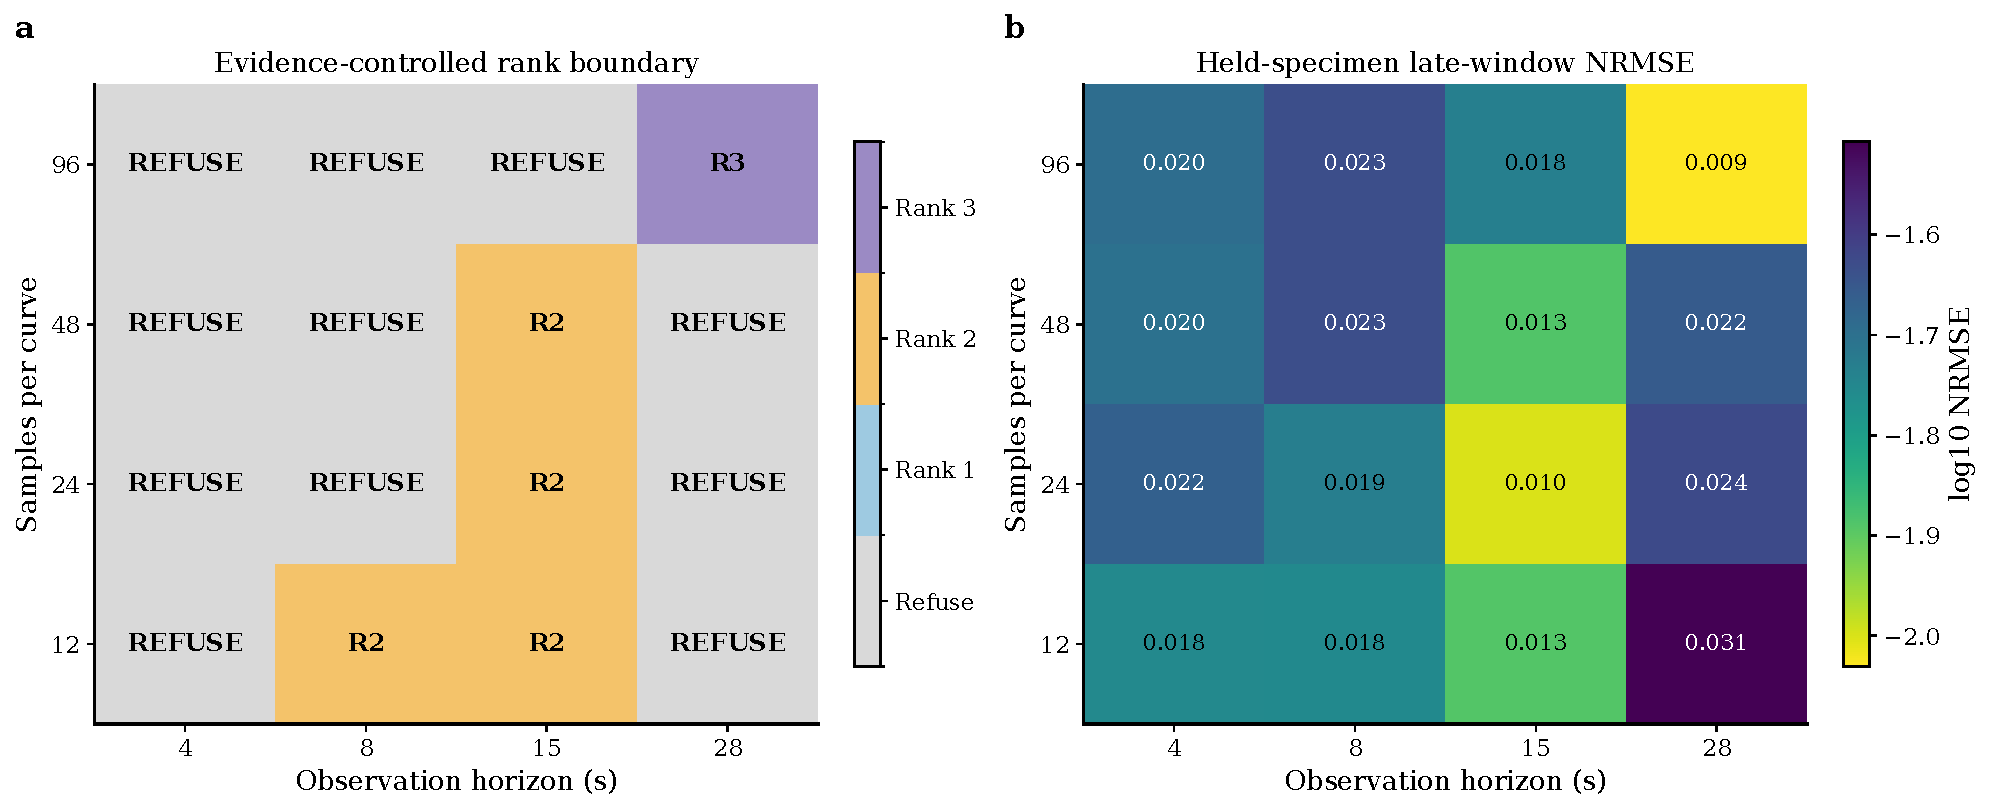
\includegraphics[width=0.94\textwidth]{fig_stage62_identifiability_boundary.pdf}
\caption{PVA 任务的观测设计边界。图中记录受支持阶数及拒绝区域，而不是在每个观测窗和采样预算下强制指定阶数。}
\label{fig:pva-boundary-zh}
\end{figure}

\subsection{铜合金支持及残差模型敏感性}
在 17 次独立应力松弛试验和 9 个留出材料组上，AR(1) 剖面 BIC 支持共享一阶经验实现。表~\ref{tab:kupfer-zh} 显示，增加模态虽然降低普通残差 BIC，却明显恶化留出材料组预测；残差相关性感知的信息准则与预测门因此共同支持一阶。普通 BIC 对更高阶的偏好作为敏感性结果保留，而不被隐藏。

\begin{table}[H]
\centering
\caption{KupferDigital 留一材料组审计。留出 NRMSE 越低越好。}
\label{tab:kupfer-zh}
\begin{tabular}{rrrr}
\toprule
阶数 & 平均 BIC & 平均 AR(1)-BIC & 留出 NRMSE 中位数\\
\midrule
1 & $-13217.40$ & $-16539.53$ & 0.3845\\
2 & $-14343.85$ & $-16512.92$ & 1.7611\\
3 & $-14468.55$ & $-16432.65$ & 104.2460\\
\bottomrule
\end{tabular}
\end{table}

所选衰减率为 3.8989 h$^{-1}$，跨折对数衰减率标准差为 0.7148，低于冻结的稳定性上限 0.8。该结果支持声明登记曲线上的紧凑共享经验松弛状态，但不能识别唯一的铜合金微观松弛机制。

\subsection{气敏预测与拒绝}
共享三阶模型在气敏恢复任务中具有较好的预测表现（表~\ref{tab:gas-zh}）。相对独立非线性拟合、固定网格 NNLS 和 Prony 递推，其实验误差中位数分别改善 26.6\%（$p=0.00110$）、80.6\%（$p<10^{-12}$）和 8.25\%（$p=0.00928$）。

\begin{table}[H]
\centering
\caption{50 次非空气气敏暴露实验的留出预测结果。}
\label{tab:gas-zh}
\begin{tabular}{lcc}
\toprule
方法 & NRMSE 中位数 & 四分位区间\\
\midrule
共享三阶 & 0.05392 & [0.03420, 0.07168]\\
独立非线性三阶 & 0.05910 & [0.05189, 0.07471]\\
固定网格 NNLS & 0.25676 & [0.20728, 0.31036]\\
Prony 递推 & 0.05961 & [0.03894, 0.08373]\\
\bottomrule
\end{tabular}
\end{table}

然而，两个三阶衰减率在约 $0.03765$ 处合并，违反式~\eqref{eq:separation-zh}，因此协议返回 \indet{}。三阶相对一阶的实验层面预测改善中位数为 65.9\%，聚类 Bootstrap 95\% 区间为 [58.5\%, 68.2\%]，但该预测优势不能修复谱的不可辨识性。全部 27 组阈值组合均保持 \indet{}，2/4/8 起点拟合也返回相同目标值和衰减率。

\begin{figure}[H]
\centering
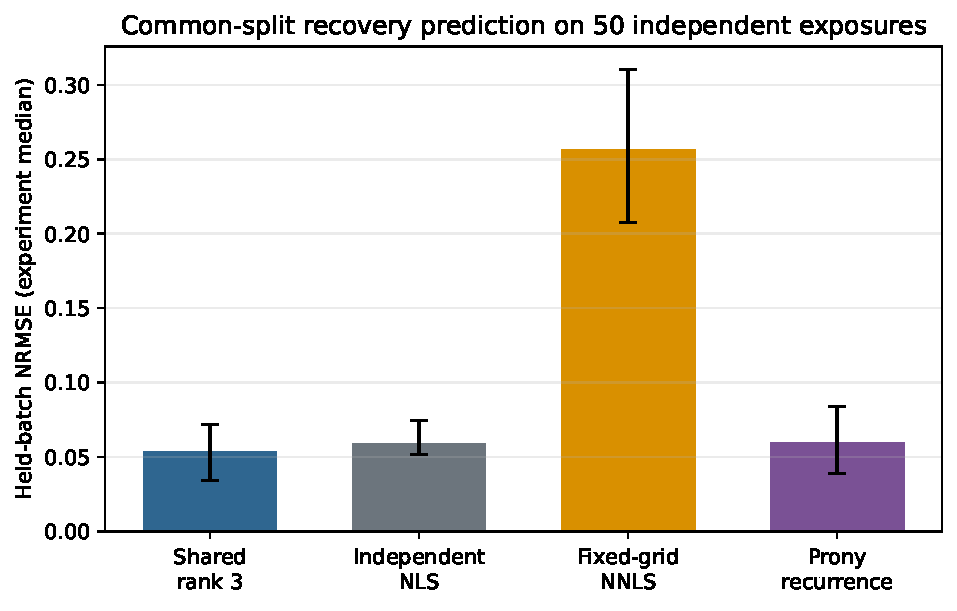
\includegraphics[width=0.94\textwidth]{fig_stage63_external_baselines.pdf}
\caption{气敏任务上的同条件外部基线。散点对应独立暴露实验，传感器通道不被计为独立重复。}
\label{fig:baselines-zh}
\end{figure}

\begin{figure}[H]
\centering
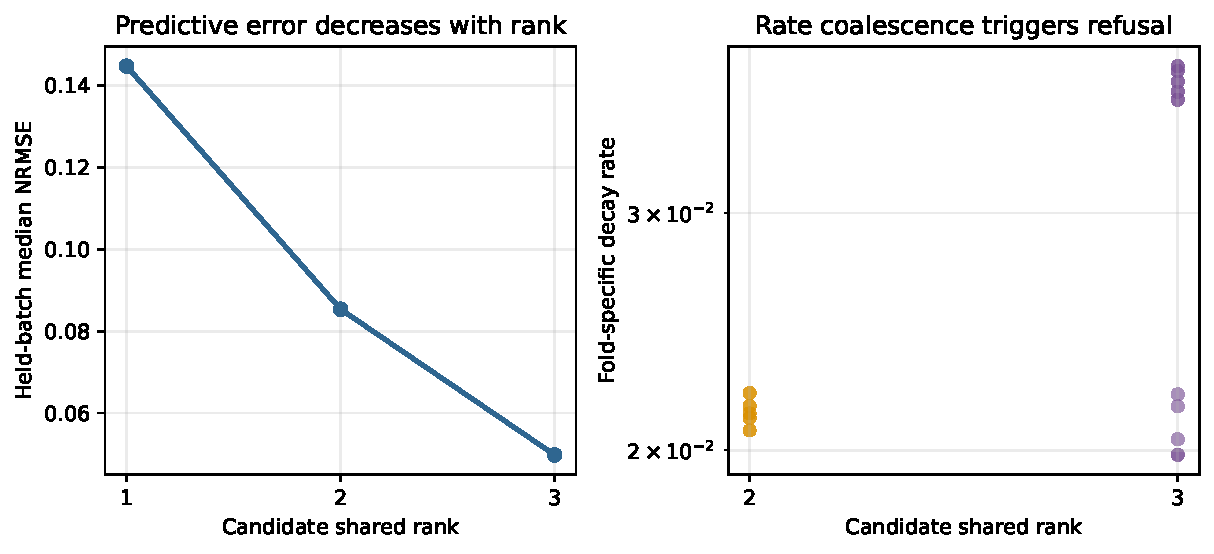
\includegraphics[width=0.94\textwidth]{fig_stage63_rank_refusal.pdf}
\caption{预测改善与拒绝判定。共享三阶模型具有较好预测性能，但衰减率分离门阻止将其解释为三个可辨识时间尺度。}
\label{fig:refusal-zh}
\end{figure}

\subsection{液压状态迁移揭示第二类拒绝}
在液压任务上，二阶模型将平均 BIC 从 $-8509.645$ 改善到 $-9167.872$，但留出循环 NRMSE 中位数由 0.23780 恶化到 0.51128。以 30 个独立循环为单位，二阶相对改善中位数为 $-73.5\%$，聚类 Bootstrap 95\% 区间为 $[-144.0\%,-38.4\%]$。其两个衰减率在下界合并，局部边界指数为 0.0571。三阶同样失败：留出循环 NRMSE 为 0.42922，完整数据的三个衰减率均在约 0.069 处合并，边界指数降至 $1.85\times10^{-7}$。全部 27 组阈值组合均输出 \indet{}。 对相关残差的敏感性分析不仅没有推翻拒绝，反而揭示准则排序不稳：普通 BIC 偏好二阶，而 AR(1) 剖面 BIC 在一阶达到最低值 $-10208.35$，二阶和三阶分别为 $-9936.23$ 与 $-9532.14$；相应平均残差 AR(1) 系数由 0.68 降至 0.49 和 0.40。

该拒绝与气敏结果不同：气敏恢复具有预测优势但缺乏谱分离；液压任务则表现为样本内信息评分改善，却无法迁移到留出部件状态且缺乏分离。二者分别触发证据契约的不同约束。

气敏任务的三个基线在 Holm 校正后的单侧配对值分别为 $2.66\times10^{-15}$（固定网格 NNLS）、0.00220（独立非线性三阶）和 0.00928（Prony），因此同任务内的预测比较结论在多重性校正后保持不变。

同切分的模型族对照也排除了仅因基线过弱而产生拒绝的解释。以独立循环为单位，共享一阶模型的 NRMSE 中位数为 0.244，拉伸指数、AR(2)、Prony 递推和固定网格 NNLS 分别为 0.329、0.316、0.491 和 0.625。在四个液压基线比较中，Holm 校正后的配对 Wilcoxon 值分别为：拉伸指数 $7.98\times10^{-4}$、Prony $6.48\times10^{-6}$、NNLS $1.20\times10^{-5}$、AR(2) 0.0249。AR(2) 的配对中位差 Bootstrap 区间跨越零，因此尽管秩检验校正值低于 0.05，该比较仍报告为混合结果。这些对照只说明声明瞬态窗口内具有预测竞争力，不支持部件级物理机制识别。

\begin{figure}[H]
\centering
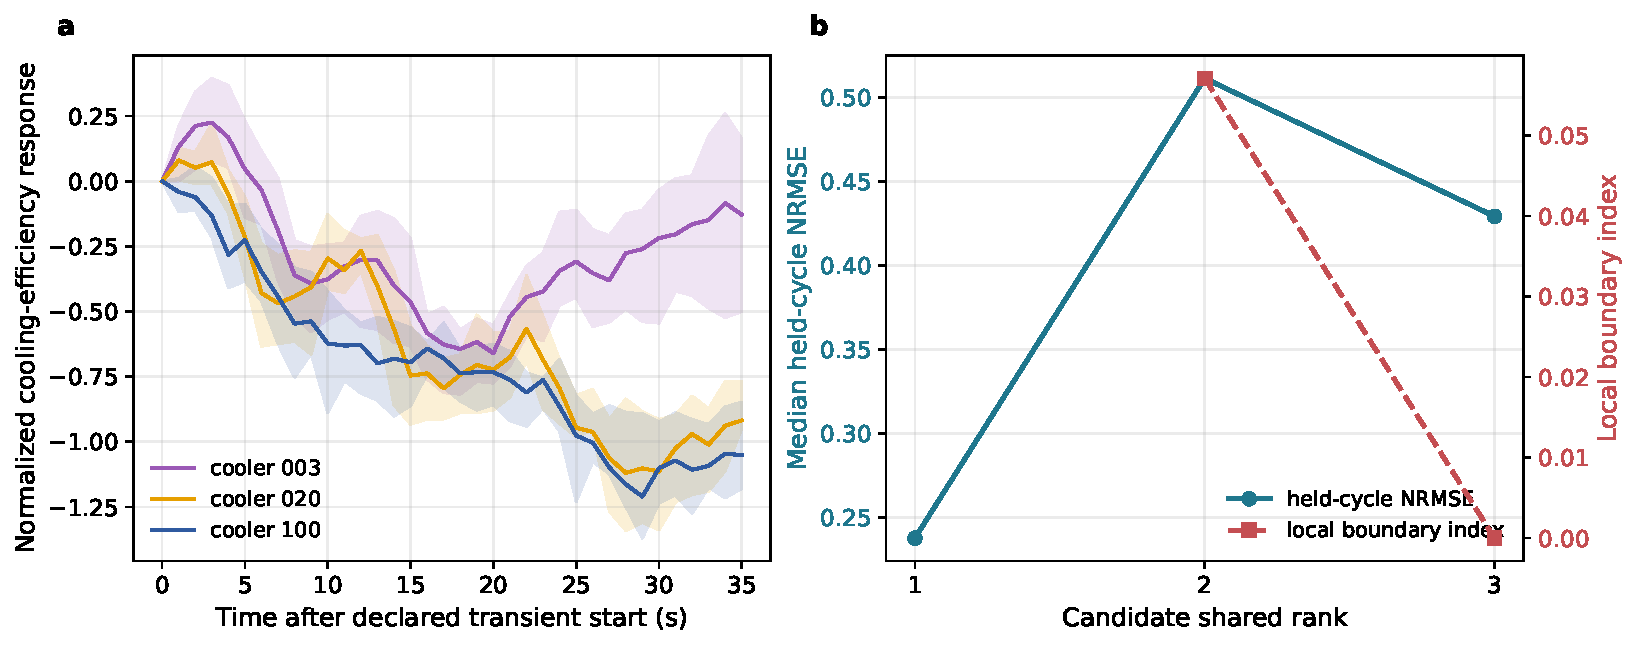
\includegraphics[width=0.96\textwidth]{fig_stage64_hydraulic_transients.pdf}
\caption{第三应用域的液压审计。（a）三种受控冷却器状态下的归一化冷却效率瞬态，阴影为独立循环的四分位区间。（b）留出循环预测误差与投影灵敏度边界诊断。后者是阶数内部的可辨识性指标，不是跨阶数性能排名。}
\label{fig:hydraulic-zh}
\end{figure}

\subsection{推荐增强组合的受控检验}
四项受控审计均使用 12 个独立种子（图~\ref{fig:extensions-zh}）。对阻尼振荡，以一个稳定共轭极点对替代三个正实极点后，留出时域 NRMSE 中位数由 0.12102 降至 0.002079，相对下降 98.3\%（单侧配对 Wilcoxon $p=2.44\times10^{-4}$），并在数值容差内恢复阻尼 0.16 和频率 2.2。在声明的组间漂移下，部分共享将 NRMSE 中位数由 0.04806 降至 0.004249（91.2\%；$p=2.44\times10^{-4}$）。对稠密对数正态松弛谱，32 点非负网格相对三阶有限模型的中位改善为 59.3\%；预先声明的 20\% 模型失配阈值在 12 个种子中的 11 个拒绝有限机制结论。该对照只诊断有限模型类不充分，不识别真实生成谱。使用 39 个独立校准组时，组级 conformal 审计在可交换对照上的平均误报率为 5.0\%，对所构造偏移备择的经验检出率为 100\%。后者只是功效观测，覆盖保证仅适用于可交换对照设计。

\begin{figure}[H]
\centering
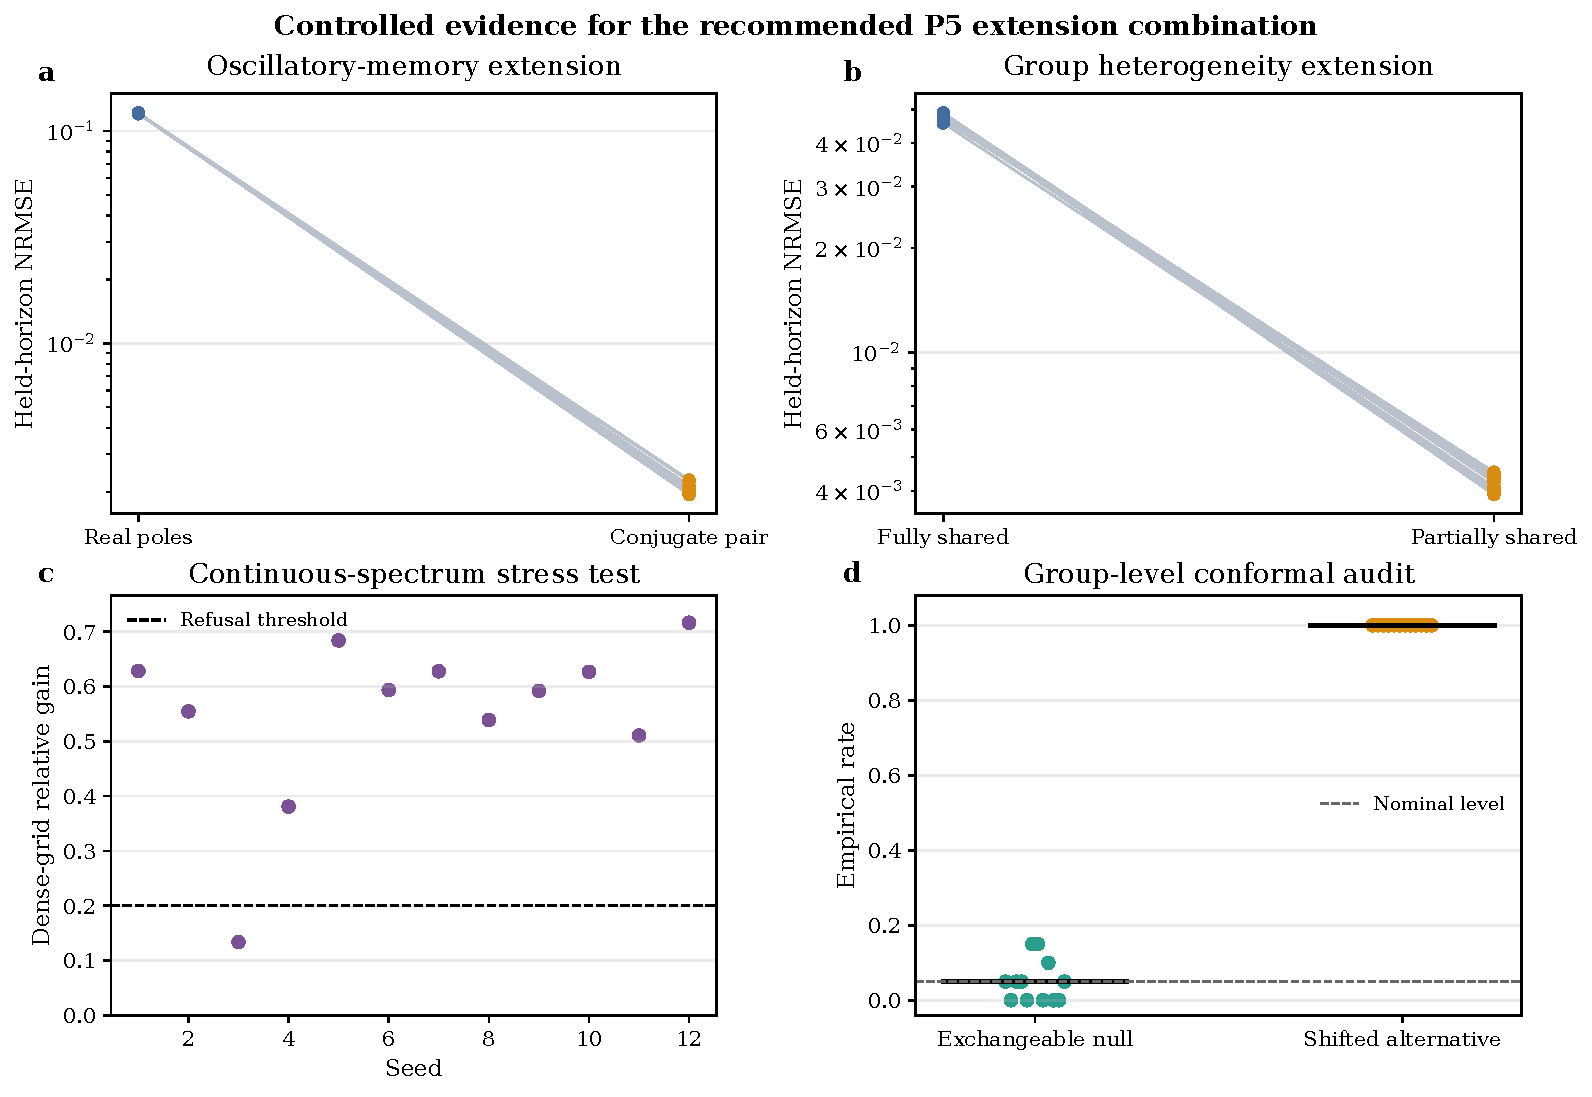
\includegraphics[width=0.96\textwidth]{fig_stage66_extension_combination.pdf}
\caption{受控扩展审计。（a）阻尼振荡上正实极点与共轭极点对的外推比较。（b）组间异质条件下完全共享与部分共享衰减率的比较。（c）稠密谱相对三阶有限模型的改善，虚线为声明的模型失配阈值。（d）组级 conformal 的误报率和偏移备择检出率。各面板只在同一受控任务内部比较方法。}
\label{fig:extensions-zh}
\end{figure}
\section{讨论}
实验结果揭示了逼近质量与机制支持之间的差别。在 PVA 数据上，跨试件预测、信息改善、衰减率稳定性和分离性在完整观测窗中一致；在铜合金数据上，留出材料预测和残差相关性感知的模型选择支持共享一阶经验状态，而仅使用普通 BIC 会给出过高阶数；在气敏数据上，预测支持更丰富的模型，但分离门否定其机制解释；在液压数据上，BIC 偏好额外模态，但迁移门和分离门共同拒绝。只报告最佳样本内或预测阶数的流程会抹去这些不同结果。

PVA 的非单调边界也表明，更长记录或更密网格不等同于单调增强的证据。增加尾部覆盖可能暴露慢模态，但相关残差会降低有效信息，更宽的衰减率范围也会恶化条件数。边界因素审计提供解释性证据而非因果定理，其目的在于指出解释阶数变化前应检验的假设。

逐门消融进一步说明协议结构：在至少一条冻结压力记录上，每个门都阻止了一次缺乏完整证据的升阶，但该诊断不量化其在未知总体中的重要性。该协议的范围有意窄于通用记忆核学习器。当前要求已声明的公共时间网格、正实衰减率、有限衰减和以及分组实验单元。主模型允许曲线特定的有符号幅值，从而可表示通道反向，但也可能产生抵消；半合成非负幅值消融并未改变“分离时支持、合并时拒绝”的结果，但这不证明任意数据上的等价性。公开数据判决仍不覆盖不规则网格和非线性状态依赖记忆。新增受控扩展证明了稳定共轭极点块、部分共享正衰减率以及稠密松弛谱下显式拒绝在计算上可行；这些结果不证明更广模型类在真实数据上的可辨识性，也不提供普适校准。在更高维算子问题中，主要成本将从标量非线性拟合转变为重复矩阵函数作用和独立参考构造。可信的扩展必须对参考误差设置预算，并保留组层级验证，而不能只扩大现有优化器。

对实践者而言，三类信号应触发拒绝或降级为较弱的表示结论：相邻衰减率低于当前设计校准的分辨率；残差相关性足以改变信息准则排序；以及样本内误差下降但留出单元性能恶化。高维辅助状态模型中的强非正规性或隐参数不可辨识会进一步放大这些问题。对于有限元、无网格或非线性 PDE，独立参考和分组留出通常主导审计成本，因此可扩展版本需要使用分层参考求解器并显式报告审计预算。

在应用上，受支持的有限实现应被理解为紧凑预测状态模型，而不是不同微观过程存在的自动证明。相反，\indet{} 也不证明多时间尺度机制不存在；它只说明冻结契约下的观测无法解析该机制。

\section{软件与可复现性}
软件包 \texttt{p5\_memory\_protocol} 冻结了四个公共操作：\texttt{fit}、\texttt{evaluate}、\texttt{decide} 和 \texttt{report}。版本化 JSON 记录保存声明域、分组单元、阈值、诊断量、判定和适用边界。以下命令可复现公开气敏任务：
\begin{verbatim}
python -m p5_memory_protocol reproduce --task uci-gas
\end{verbatim}
在本稿整理时，151 项单元测试全部通过，76 个机器可读结果文件均可解析。这些检查证明内部可复现性；外部团队独立复现仍是另一项要求。

\section{结论}
本文提出一种证据门控方法，用于识别最小受支持共享有限记忆实现，并主动拒绝缺乏证据的阶数结论。正式的相邻衰减率边界说明何时不存在一致阶数检验；独立推论则在明确的校准、估计一致性和固定分离条件下给出拒绝或接受结论。四个公开应用域给出互补结果：完整观测窗的 PVA 应力松弛支持三阶有限经验实现；铜合金应力松弛在残差相关性感知的模型选择和留出材料预测下支持共享一阶经验状态；气敏恢复预测较好但无法解析相邻模态；液压冷却瞬态改善普通 BIC，却不能迁移到留出部件状态。受控扩展进一步表明，同一证据纪律可以容纳稳定振荡模态和部分共享，也能在稠密谱下拒绝有限机制结论，且不改变四个公开数据任务的判决。由此形成一套有明确适用范围的统计与计算协议，用于区分有用表示与过度解释的机制结论。

\section*{数据与代码可用性}
公开源数据集的 DOI 已列于参考文献。派生结果、协议定义、测试和图片生成脚本保存在项目目录中。仓库地址和归档软件 DOI 仅在冻结的公开版本完成核验后写入。

\section*{CRediT 作者贡献声明}
\textbf{段海涛：}概念构建、方法、软件、形式分析、研究、验证、初稿撰写、审阅与修改。\textbf{胡宁：}概念构建、方法、监督、数据整理、验证、可视化、审阅与修改。\textbf{李书群：}研究、验证、形式分析、审阅与修改。\textbf{胡初扬：}研究、验证、软件核验、审阅与修改。

\section*{基金资助}
本研究得到上海交通大学海洋工程国家重点实验室（项目编号 GKZD010089）和中国科学院声学研究所声学与海洋信息全国重点实验室（项目编号 SKLA202406）的资助。资助方未参与研究设计、数据收集、分析与解释、稿件撰写或投稿决定。

\section*{利益冲突声明}
作者声明不存在可能影响本文工作的已知竞争性经济利益或个人关系。

\section*{生成式人工智能与人工智能辅助技术声明}
稿件准备过程中，作者使用人工智能辅助工具进行语言编辑、文档组织和一致性检查。作者对生成内容、数值论断、代码输出和参考文献进行了审阅与核验，并对稿件内容承担全部责任。

\section*{伦理声明}
本研究使用公开的非人类数据集和合成数值实验，不涉及人类受试者、可识别个人数据或动物实验。

\section*{作者标识符}
段海涛：ORCID 0009-0006-4611-8639；胡宁：ORCID 0000-0002-2718-0385；李书群：ORCID 0009-0007-1787-685X；胡初扬：ORCID 0009-0007-9255-018X。

\bibliographystyle{unsrt}
\bibliography{references}
\end{document}






